\documentclass{article}

\usepackage{graphicx}
\usepackage{tikz}
\usepackage{tikzsymbols}
\usetikzlibrary{calc,patterns,shapes.geometric}
\pagestyle{empty}
\usepackage[margin=0pt]{geometry}
\geometry{papersize={14in,12in}}

\def\centerarc[#1](#2)(#3:#4:#5){\draw[#1] ($(#2)+({#5*cos(#3)},{#5*sin(#3)})$) arc (#3:#4:#5);}

\begin{document}
	\begin{figure}
		\centering
		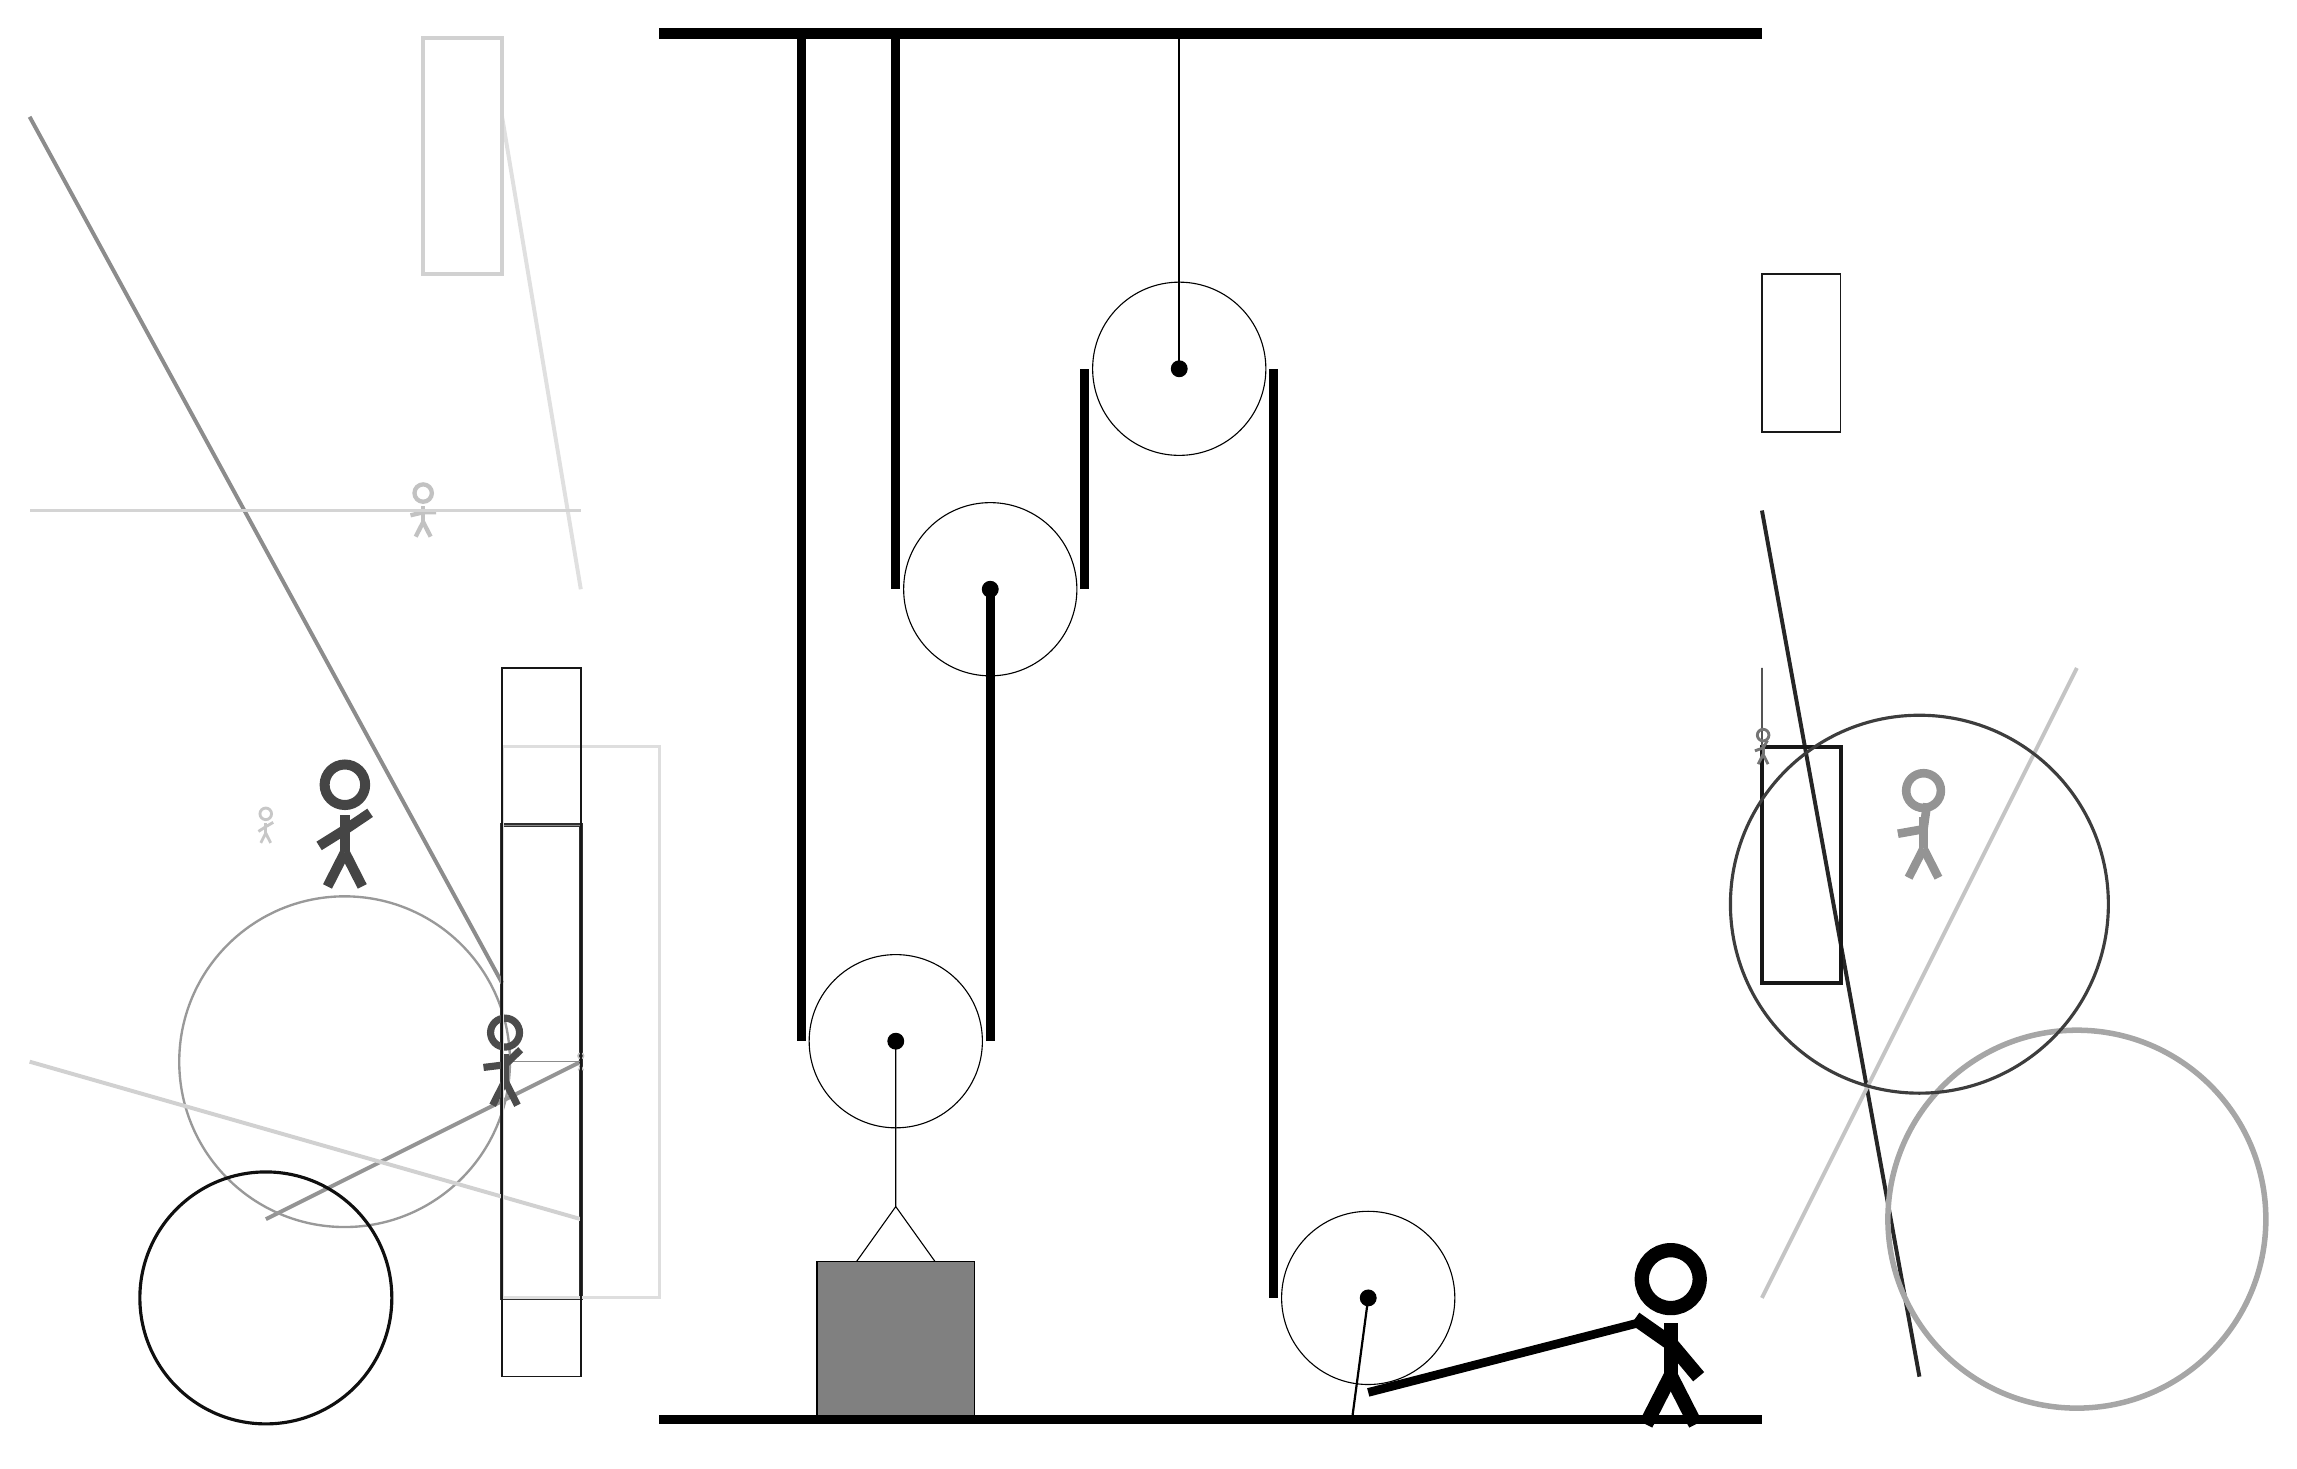
\begin{tikzpicture}
			%%%%% START %%%%%
			
			\draw[fill=black] (-2, 14) rectangle (12, 14.125);
			
			\draw (1, 1.26) circle (1.1);
			\draw[fill=black] (1, 1.26) circle (0.1);
			
			\draw (2.2, 7.0) circle (1.1);
			\draw[fill=black] (2.2, 7.0) circle (0.1);
			
			\draw (4.6, 9.8) circle (1.1);
			\draw[fill=black] (4.6, 9.8) circle (0.1);
			\draw[thick] (4.6, 9.8) -- (4.6, 14);
			
			\draw (7.0, -2) circle (1.1);
			\draw[fill=black] (7.0, -2) circle (0.1);
			\draw[thick] (7.0, -2) -- (6.8, -3.5);
			
			\node[line width=0.2mm, color=black!24] at (-5, 8) {\Strichmaxerl[3][13][1]};
			
			\draw[line width=0.5mm, color=black!85](12, 8) -- (14, -3);
			\draw[line width=0.5mm, color=black!42](-7, -1) -- (-3, 1);
			\node[line width=0.7mm, color=black!42] at (14, 4) {\Strichmaxerl[6][10][82]};
			\draw [line width=0.3mm, color=black!40](-6, 1) circle (2.1);
			\draw[line width=0.5mm, color=black!91] (13, 5) rectangle (12, 2);
			
			\draw[line width=0.5mm, color=black!81] (-4, 4) rectangle (-3, -2);
			\draw[line width=0.3mm, color=black!67] (12, 6) rectangle (12, 5);
			\draw[line width=0.2mm, color=black!90] (13, 9) rectangle (12, 11);
			\draw[line width=0.5mm, color=black!12](-3, 7) -- (-4, 13);
			
			\draw[line width=0.5mm, color=black!18] (-4, 11) rectangle (-5, 14);
			\draw[line width=0.2mm, color=black!45] (-4, 4) rectangle (-3, 1);
			\draw[line width=0.5mm, color=black!18](-3, -1) -- (-10, 1);
			
			\draw[line width=0.5mm, color=black!23](12, -2) -- (16, 6);
			\draw [line width=0.7mm, color=black!35](16, -1) circle (2.4);
			\node[line width=0.7mm, color=black!70] at (-4, 1) {\Strichmaxerl[5][7][44]};
			
			\node[line width=0.4mm, color=black!24] at (-3, 1) {\Strichmaxerl[1][66][87]};
			
			\node[line width=0.5mm, color=black!22] at (-7, 4) {\Strichmaxerl[2][33][30]};
			\draw[line width=0.4mm, color=black!13] (-2, -2) rectangle (-4, 5);
			
			\draw [line width=0.4mm, color=black!94](-7, -2) circle (1.6);
			\draw [line width=0.4mm, color=black!76](14, 3) circle (2.4);
			
			\draw[line width=0.5mm, color=black!45](-4, 2) -- (-10, 13);
			
			\draw[line width=0.5mm, color=black!17](-3, 8) -- (-10, 8);
			\node[line width=0.7mm, color=black!54] at (12, 5) {\Strichmaxerl[2][19][60]};
			\draw[line width=0.2mm, color=black!91] (-4, -3) rectangle (-3, 6);
			
			\node[line width=0.4mm, color=black!73] at (-6, 4) {\Strichmaxerl[7][32][34]};
			
			
			\draw (1, 1.26) -- (1, -0.84) -- (0.5, -1.54) -- (1.5, -1.54) -- (1, -0.84);
			\draw[fill=black!50] (0, -1.54) rectangle (2, -3.54);
			\draw[line width=1.1mm] (-0.2, 14) -- (-0.2, 1.26);
			\centerarc[line width=1.1mm](1, 1.26)(180:360:1.2000000000000002);
			\draw[line width=1.1mm](2.2, 1.26) -- (2.2, 7.0);
			\draw[line width=1.1mm] (1.0, 14) -- (1.0, 7.0);
			\centerarc[line width=1.1mm](2.2, 7.0)(180:360:1.2000000000000002);
			\draw[line width=1.1mm](3.4, 7.0) -- (3.4, 9.8);
			\centerarc[line width=1.1mm](4.6, 9.8)(0:180:1.2000000000000002);
			\draw[line width=1.1mm] (5.8, 9.8) -- (5.8, -2);
			\centerarc[line width=1.1mm](7.0, -2)(0:90:-1.2000000000000002);
			\draw[line width=1.1mm](7.0, -3.2) -- (10.5, -2.3);
			
			\node at (10.8, -2.5) {\Strichmaxerl[10][-35][-50]};
			
			\draw[fill=black] (-2, -3.5) rectangle (12, -3.6);
			
			%%%%% END %%%%%
		\end{tikzpicture}
	\end{figure}	
\end{document}